\documentclass[12pt,fleqn]{article}
\usepackage{../lecture-notes/vkCourseML}
%\usepackage{vkCourseML}
\usepackage{lipsum}
\usepackage{indentfirst}
\usepackage{graphicx}
\usepackage{animate}
\usepackage{hyperref}
\graphicspath{{./figures/}}
\title{Машинное обучение, ФКН ВШЭ\\Семинар №21}
\author{}
\date{}

\begin{document}
\maketitle



\section{Multi-label классификации}

В классической задаче многоклассовой классификации необходимо каждому объекту сопоставлять метку одного из классов, к которому этот объект принадлежит. На практике также встречаются задачи, где объект может принадлежать сразу нескольким классам. Такие задачи называют задачами классификации с пересекающимися классами~(multi-label classification). Такие задачи встречаются, например, в задаче категорирования новостей, тегирования песен и изображений. Рассмотрим подходы к решению таких задач.

\subsection{Multi-label задача как множество независимых задач бинарной классификации}

В простом случае можно рассматривать каждую метку независимо, то есть решать задачу бинарной классификации "соответствует ли конкретный объект заданной метке". В таком случае необходимо обучить столько классификаторов, сколько меток существует в нашей задаче. Однако простота решения задачи как множество независимых задач оборачивается тем, что мы теряем связь между метками. Например, знание о том, что фильм является ужастиком, может сильно поменять предсказание "является ли фильм романтическим": $p(y_{\mbox{romance}} | x) \ne p(y_{\mbox{romance}} | x, y_{\mbox{horror}})$.

Упрощение модели можно представить аналогично наивному байесовскому классификатору (только факторизуем распределение не по признакам, а по меткам):

$$
p(y_1, y_2, \dots, y_D | x) \approx \prod_{i=1}^{D} p(y_i | x)
$$

Тогда предсказание каждой метки:

$$
\hat{y_i} = \argmax_{y_i} p(y_i | x)
$$

\subsection{Моделирование зависимостей между метками}

Используя определение условной вероятности, можно получить следующее соотношение:

$$
p(y_1, y_2, \dots, y_D | x) = \prod_{i=1}^{D} p(y_i | x, y_1, y_2, \dots, y_{i - 1})
$$

Оно соответствует модели на рис. (\ref{fig:graph}).

\begin{center}
\begin{figure}[!htb]
 \centering
 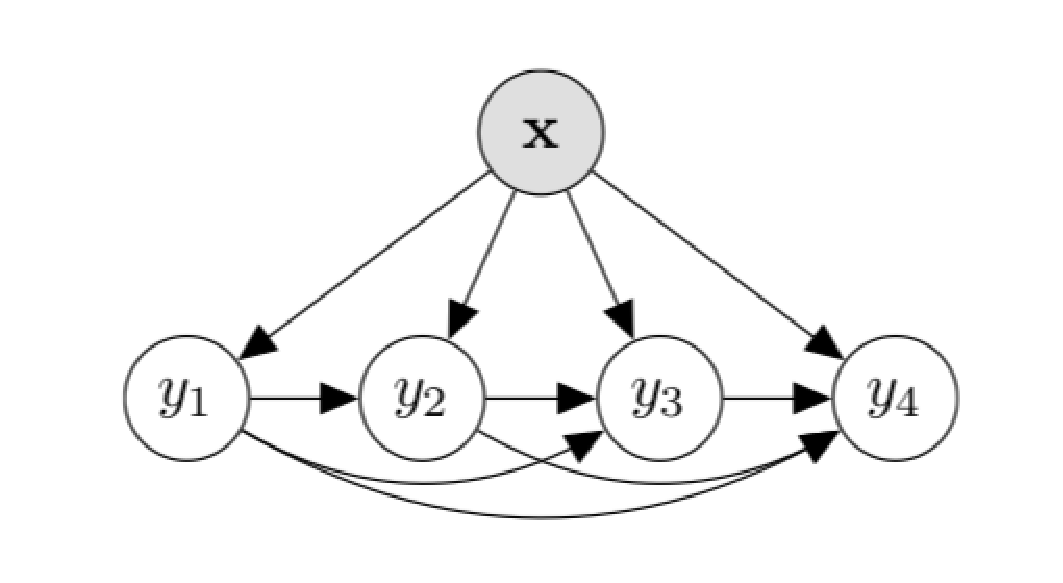
\includegraphics[width=0.5\linewidth]{graph.eps}
 \caption{Моделирование зависимостей между метками}\label{fig:graph}
\end{figure}
\end{center}

При таком подходе предсказания нельзя получить независимо по меткам как в предыдущем случае. Существует несколько подходов:

\begin{enumerate}
    \item Жадный подход заключается в последовательном применении $\argmax_{y_i}$ в порядке всех меток. Решение может быть далёким от оптимального, но требует минимального числа вычислений.
    \item Оптимальный подход заключается в расчёте всех вероятностей $p(y_1, y_2, \dots, y_D | x)$ с последующим применением $\argmax$ к совместном распределению (получится дерево всех возможных значений меток, где в листьях будут вероятности возможных $\hat{y}$). Число вершин будет расти экспоненционально, поэтому такой способ применим только в задачах с малым количеством меток ($\approx 15$).
    \item Beam-search заключается в обогащении жадного подхода поддержкой не одного значения --- текущего $\argmax$, а сразу нескольких на случай, если путь с максимальной вероятностью на конкретном шаге не будет оптимальным в итоге.
    \item Монте-Карло подход заключается в сэмплировании, по какому пути дерева пойти дальше.
\end{enumerate}

С точки зрения обучения моделей и матрицы признаков это будет выглядеть так, что алгоритм получает для обучения матрицу признаков и метки или предсказания всех предшествующих меток. В таком случае нужно быть аккуратным и не допустить переобучения, подавая ответы на предшествующих метках следующим алгоритмам в качестве признаков (как это случается в стэкинге).

Сложностью этого подхода является то, что необходимо выбрать порядок меток, так как на практике мы делаем оценки на эти распрееления и формальное равенство распределений для любого порядка меток будет нарушаться. Также иногда можно исключить некоторые метки из условных распределений с правой стороны, если есть информация о том, что они не влияют на распределение (особенно, если в задаче много меток).

\subsection{Label Powerset}

Все метки --- бинарные величины. Можно представить множество меток как двоичное число и тем самым свести задачу к задаче многоклассовой классификации. Например, для задачи предсказания 4 меток объект с метками 0|1|1|0 будет представлен как класс 6 ($0 * 8 + 1 * 4 + 1 * 2 + 0 * 1$).

Однако мы получим задачу с большим количеством классов, многие из которых похожи друг на друга (отличие у двух объектов в одной метке разносит их в разные классы), но для модели будут являться разными. Заметим, что на самом деле у нас вряд ли будет $2^D$ классов, так как в выборке не будут встречаться некоторые сочетания меток (то есть такие сочетания меток и не смогут быть предсказанными моделью).

Для борьбы с большой размерностью целевой переменной можно делать такое преобразование для подмножества меток размерности $k$ (метод RAkEL). Для каждого подмножества будет решаться отдельная задача многоклассовой классификации, а итоговое предсказание меток можно делать голосованием этих моделей (все модели, в подмножество меток которых попало конкретная метка, предскажут на основе своих классов бинарные метки для конкретной метки, среди которых можно произвести голосование).

В реальных задачах часто можно предполагать, что некоторые метки можно объедить в кластера по их смыслу. В таком случае можно произвести кластеризацию меток на $k$ кластеров и предсказывать принадлежность объекта сразу группе меток на первом уровне, далее предсказывать отдельные метки внутри каждого кластера (например, произвести кодирование в задачу многоклассовой классификации).

Также можно искать связи между метками, считая взаимную информацию между метками или совместные распределения.

\subsection{Отображение меток в пространство меньше размерности}

При решении $D$ независимых задач бинарной классификации сильно растут накладные расходы из-за количества меток и теряется связь между метками. В случае кодирования задачи в задачу многоклассовой классификации число классов растёт экспоненциально. Альтернативный вариант заключается в построении отображения меток в пространство меньшей размерности с дальнейшим решением независимых задач по каждой координате нового пространства. Предсказания модели в таком случае необходимо отображать обратно в исходное пространство.

Один из способов получить проекционную матрицу является сингулярное разложение\footnote{\href{http://ntur.lib.ntu.edu.tw/retrieve/188514/18.pdf}{Multi-label Classification with Principle Label Space Transformation}}. Разложим матрицу меток:

$$
Y = U \Sigma V^\top
$$

Возьмём первые $m$ столбцов ($m \ll D$), соответствующие наибольшим собственным числам, в матрице $U$ --- $\hat{U}$. Так как $U$ унитарная матрица, то $U^\top$ -- проекционная матрица для пространства меток ($U^\top Y = \Sigma V^\top$). $\hat{U}$ -- наилучшая проекционная матрица в размерность $m$ (при восстановлении получим наименьшую квадратичную ошибку).

Перейдём в новое пространство $\hat{Y} = \hat{U^\top} Y$, в котором будем решать регрессионную задачу размерности $m$. Предсказания будем отображать обратно, умножая слева на $\hat{U}$. Из-за меньше размерности $m \ll D$ получим более простую задачу, при этом косвенно найдём близкие по смыслу метки (в рамках сингулярного разложения).

Можно также вместо сингулярного разложения использовать произвольную проекционную матрицу, однако будет необходимод найти для неё обратный переход в исходное пространство.


\subsection{Сведение известных методов к multi-label классификации}

Некоторые из алгоритмов машинного обучения можно модифицировать для решения задачи multi-label классификации, при этом усложнить его не пропорционально количество меток (как в случае сведения к задаче бинарной классификации). Рассмотрим несколько методов.

\begin{enumerate}
	\item Метод k-ближайших соседений. Для $k$ ближайших соседей можно посчитать долю объектов, принадлежащей каждой метке: $p(y_i = 1 | x) = \frac{1}{k} \sum_{j \in {N_k}} y_i^{(j)}$.

	\item Нейронные сети. Гибкость нейронных сетей позволяет получить такой выход из модели, который нужен в конкретной задаче. В multi-label классификации можно сделать на последнем слое нейронной сети по нейрону на каждую метку с сигмоидальной функцией активации. В таком случае модель будет решать задачу бинарной классификации для каждой из меток, однако число параметров сети вырастет пропорционально количеству меток только на последнем слое.

    \item Решающие деревья. Можно модифицировать дерево так, чтобы критерий информативности был соответствовал multi-label задаче и в листьях делалось предсказание для каждой из меток (аналогично методу $k$ ближайших соседей).
\end{enumerate}

\subsection{Подбор порога бинаризации}

Иногда в реальных задачах нужно бинаризовать предсказанные вероятности для получения меток. Это можно делать несколькими способами:

\begin{enumerate}
    \item Общий порог 0.5 для всех меток.
    \item Подбор порога для каждой метки такой, чтобы доля положительных объектов на тесте была такой же, как в обучающей выборке.
    \item Подбор порога для каждой метки с учётом некоторой функции потерь.
\end{enumerate}

\section{Focal loss}

Рассмотрим подход с модификацией функции потерь, предложенный в статье \footnote{Focal Loss for Dense Object Detection, \href{https://arxiv.org/pdf/1708.02002.pdf}{arxiv:1708.02002}} про детекцию изображений. Важной частью всех детекторов изображений является решение задачи классификации для большого количества участков изображения. При этом многие из этих участков (патчей) содержат только фон, то есть преобаладает класс "фон". Многие из изображений фона легко классифицируются как фон. То есть возникает много примеров одного из классов, которые при этом и так легко классифицируются моделью. Из-за этого при обучении под кросс-энтропийный критерий мы неэффективно учимся. Мы не будем вдаваться в подробности устройства детекторов изображений и особенностей их обучения, а сконцентрируемся на задаче классификации.

Классическую кросс-энтропийную функцию потерь в задаче бинарной классификации можно записать следующим образом:

$$
CE(y, p) = \begin{cases} - \log (p), & \mbox{if } y = 1 \\ - \log (1-p), & \mbox{if } y = 0 \end{cases}
$$

Для удобства введём обозначение:

$$
p_t = \begin{cases} p, & \mbox{if } y = 1 \\ 1 - p, & \mbox{if } y = 0 \end{cases}
$$

В таком случае получим $CE(y, p) = CE(p_t) = - \log (p_t)$. В случае, когда $p_t \gg 0.5$ объект классифицируется правильно, ошибка хоть и мала, но всё ещё ненулевая, а в случае большого количества простых для классификации примеров преобладающий класс может "задавить" более редкий в функции потерь. Модель будет учиться для этих объектов предсказывать всё более близкие к 1 вероятности вместо того, чтобы лучше классифицировать объекты более редкого класса.

Одним из вариантов борьбы с эффектом несбалансированных классов является добавление балансирующего коэффициента. В таком случае $CE(p_t) = - \alpha_t \log p_t$, где

$$
\alpha_t = \begin{cases} \alpha, & \mbox{if } y = 1 \\ 1 - \alpha, & \mbox{if } y = 0 \end{cases}
$$

$$\alpha \in (0, 1)$$

Обычно этот коэффициент пропорционален балансу классов и, таким образом, в функции потерь объекты редкого класса начинают "весить" столько же, сколько и объекты популярного класса.

Однако в этом случае всё ещё "лёгкие" для модели объекты из-за своего количества могут перебивать "сложные" примеры. Можно модифицировать исходную формулу добавлением коэффициента, зависящего от предсказаний:

$$FL(p_t) = - (1 - p_t)^\gamma \log p_t, \gamma \in [0, 5]$$.

При $\gamma = 0$ это всё ещё стандартная кросс-энтропийная функция потерь, а для других значений получаем, что вес объекта зависит от того, насколько модель уверена в своих предсказаниях. В таком случае при обучении модель будет меньше стремиться "дотюниваться" под популярные и "лёгкие" примеры. Также можно использовать коэффициент для баланса между классами: $FL(p_t) = - \alpha_t (1 - p_t)^\gamma \log p_t$.

\begin{center}
\begin{figure}[!htb]
 \centering
 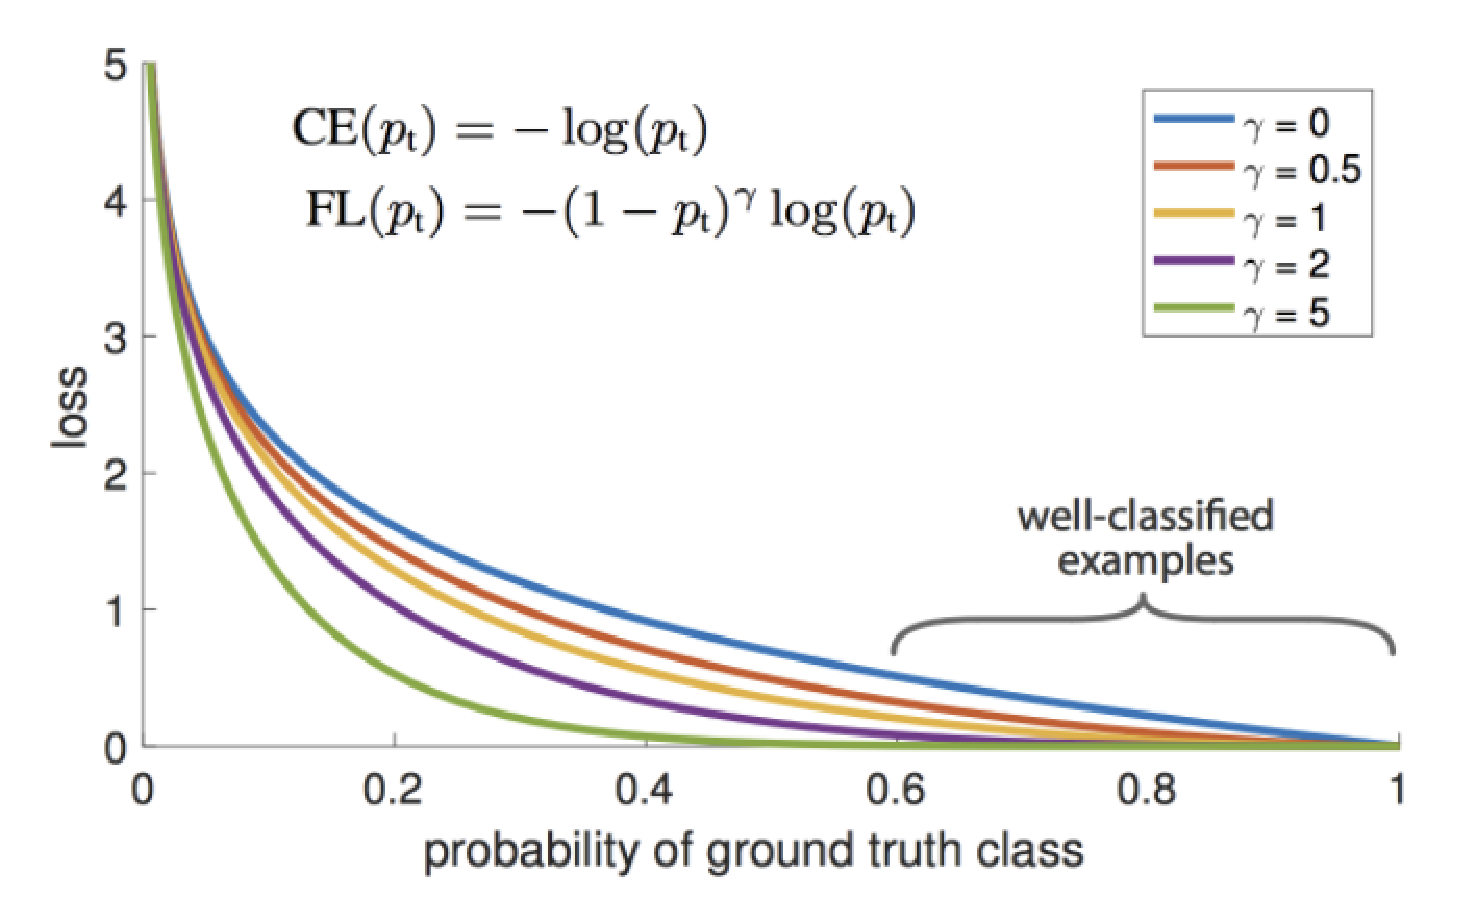
\includegraphics[width=0.7\linewidth]{focal_loss.eps}
 \caption{Вид focal loss для различных значений $\gamma$}\label{fig:plot}
\end{figure}
\end{center}

На рис. (\ref{fig:plot}) представлен вид focal loss для различных значений параметра $\gamma$ и кросс-энтропийная функция потерь. Можно увидеть, что в правой части графика, когда модель уверена в предсказаниях, штраф тем меньше, чем больше $\gamma$.



\end{document}
